\documentclass[dvipdfmx]{jsarticle}
\usepackage{amsmath,amssymb}
\usepackage{color}
\usepackage[hiresbb]{graphicx}
\usepackage{here}
\usepackage{bm}
\newcommand{\average}[1]{\ensuremath{\langle#1\rangle} }
\newcommand{\point}{\textcircled{\textcolor{red}{\scriptsize キ}} }
\newcommand{\proof}{\textcircled{\textcolor{blue}{\scriptsize P}} }
\newcommand{\defEq}{\overset{\mathrm{def}}{\Leftrightarrow}}
\newcommand{\opensubset}{\underset{open}{\subseteq}}
\newcommand{\closedsubset}{\underset{closed}{\subseteq}}


\begin{document}
\section{連続写像}
\begin{description}
    \item[\bf{Definition:}] 連続写像$f : X \mapsto Y$
        \begin{itemize}
            \item $X = I \subset \mathbb{R},\ Y = \mathbb{R}$ (実数値連続関数)
                $$ \forall x_0 \in X,\ \lim_{x \to x_0} f(x) = f(x_0) $$
                $\epsilon-\delta$記法では, 
                $$ \forall x_0 \in X,\ \forall \epsilon > 0,\ \exists \delta > 0,\ ( \forall x \in X : |x - x_0 | < \delta ),\ | f(x_0) - f(x) | < \epsilon $$
            \item $X, Y$が距離空間
                $$ \forall x_0 \in X,\ \forall \epsilon > 0,\ \exists \delta > 0,\ ( \forall x \in X : d_X(x,\ x_0) < \delta),\ d_Y(f(x_0),\ f(x)) < \epsilon $$
                $x_0 \in X$は, 孤立点または集積点に分類される.
                \begin{itemize}
                    \item $x_0$が孤立点のとき, $f$は$x_0$において常に連続.
                    \item $x_0$が集積点のとき, $f$は$x_0$において連続であるとは, 
                        $$ \displaystyle \lim_{ x \in X - \{ x_0 \} ,\ x \to x_0} f(x) = f(x_0) $$
                \end{itemize}
            \item $X, Y$が位相空間 \\
                開集合を用いた定義
                $$ \forall Q \underset{open}{\subseteq} Y,\  f^{-1}(Q) \underset{open}{\subseteq} X$$
                閉集合を用いた定義
                $$ \forall Q \underset{closed}{\subseteq} Y,\  f^{-1}(Q) \underset{closed}{\subseteq} X$$
        \end{itemize}
    
    \item[\bf{Theorem:}] コンパクト空間の連続像
    \begin{center}$X$がコンパクト位相空間, $f : X \mapsto Y$が連続写像 $\Rightarrow$ $f(X)$はコンパクト位相空間. \end{center}
        \point : 連続写像はコンパクト性を保つ. \\
        \begin{proof}
            $f(X)$の任意の開被覆に対して有限の部分開被覆が取れることを示す.
        \end{proof}

    \item[\bf{Theorem:}] 最大最小値の定理
        \begin{itemize}
            \item 実連続写像$f : [a,\ b] \mapsto \mathbb{R}$
            \begin{center}$f([a,\ b])$は最大値と最小値をもつ.\end{center}
            \item 実連続写像$f: X \mapsto \mathbb{R}$, $X$がコンパクト空間 
            \begin{center}$f(X)$は最大値と最小値をもつ.\end{center}
        \end{itemize}
        \begin{proof}
            $f(X)$はコンパクト空間, コンパクト空間には最大値と最小値が存在.
        \end{proof}

    \item[\bf{Theorem:}] 連結空間の連続像
        \begin{center} $X$が連結位相空間, $f : X \mapsto Y$が連続写像 $\Rightarrow$ $f(X)$は連結位相空間. \end{center}
        \point : 連続写像は連結性を保つ. $X \subset \mathbb{R}$のとき, $\mathbb{R}$の部分連結空間は区間より, $f(X)$は区間となる. \\
        \begin{proof}
            分離開集合$f(X) \subseteq U \cup V$が取れると分離開集合$X = f^{-1}(U) \cup f^{-1}(V)$が取れて矛盾.
        \end{proof}
        
    \item[\bf{Theorem:}] 中間値の定理
        \begin{itemize}
            \item 実連続写像$f : [a,\ b] \mapsto \mathbb{R},\ f(a) = \alpha,\ f(b) = \beta,\ \alpha < \beta$
                $$ (\forall \gamma \in \mathbb{R}: \alpha < \gamma < \beta),\ (\exists c \in [a,\ b] : f(c) = \gamma) $$

            \item 実連続写像$f: X \mapsto \mathbb{R}$, $X$が連結空間, $a,\ b \in X,\ f(a) = \alpha,\ f(b) = \beta,\ \alpha < \beta$\\
            $$ (\forall \gamma \in \mathbb{R}: \alpha < \gamma < \beta),\ (\exists c \in X : f(c) = \gamma) $$
        \end{itemize}
        \begin{proof}
            $f(X) \subseteq \{ f(x) \mid f(x) < \gamma \} \cup \{ f(x) \mid f(x) > \gamma \}$となると$f(X)$が連結という事実に矛盾.
        \end{proof}
    
    \item[\bf{Theorem:}] 連続写像の合成
        \begin{center}$f: X \mapsto Y,\ g: Y \mapsto Z$が連続写像 $\Rightarrow$ $g \circ f : X \mapsto Z$ も連続写像. \end{center}
        \begin{proof}
            $(g \circ f)^{-1}(A) = g^{-1}(f^{-1}(A)) \underset{open}{\subseteq} X$
        \end{proof}
    
    \item[\bf{Definition:}] 一様連続写像 $f : X \mapsto Y$ \\
        \point : $x_0$の位置によらず, 同じ$\delta$で抑えられる.
        \begin{itemize}
            \item $X = I \subset \mathbb{R},\ Y = \mathbb{R}$ (実数値連続関数)
                $$ \forall \epsilon > 0,\ \exists \delta > 0,\ { \color{red} \forall x_0 \in X},\ ( \forall x \in X : |x - x_0 | < \delta),\ | f(x_0) - f(x) | < \epsilon $$
            \item $X, Y$が距離空間
            $$ \forall \epsilon > 0,\ \exists \delta > 0,\ { \color{red} \forall x_0 \in X},\ ( \forall x \in X : d_X(x,\ x_0) < \delta),\ d_Y(f(x_0),\ f(x) ) < \epsilon $$
        \end{itemize}
    
    \item[\bf{Theorem:}] 連続写像が一様連続写像である1つの条件
        \begin{center} 連続写像$f : X \mapsto Y$について, $X$がコンパクト空間のとき$f$は一様連続写像 \end{center}
        \point コンパクト空間からの連続写像は, コンパクト性を保存かつ一様連続. \\
        \begin{proof} 証明
            \begin{enumerate}
                \item $\epsilon > 0$を決める.$\forall c \in X,\ d(f(c),\ f(x)) < \epsilon$を満たす$x$の動ける範囲$B(c,\ \delta(c))$を求める.
                \item $ X \subseteq \cup_{c \in X} B(c,\ \delta(c)) \underset{conpact}{\Rightarrow} X \subseteq \cup_{i = 0}^{n} B(c_i,\ \delta(c_i))$
                \item $\delta = \min_{i=1 .. n} \delta(c_i)$ として決めると, \\
                $\forall x_* \in X,\ d( x_*,\ x) < \delta $ を満たすとき, $x,\ x_*$は2点ともどこかの開球に入る.
            \end{enumerate}
        \end{proof}
    \item[\bf{Example:}] 連続写像だが一様連続写像でない例
        $$ f(x) = x^2 \ ( x \in \mathbb{R}) $$
        $a > 0$とすれば, 
        $ | x^2 - a^2 | = | (x-a) (x+a) | \leq | x - a || x + a| = |x-a||x-a+2a| \leq |x-a|(|x-a|+2a)$ より, $\delta = a \wedge \frac{\epsilon}{3a} $とすれば, 
        $ | x^2 - a^2 | \leq |x-a|(|x-a|+2a) \leq \frac{\epsilon}{3a}(2a + a) = \epsilon $となる.

    \item[\bf{Definition:}] 同相写像(位相同形写像)
        \begin{center}連続写像$f: X \mapsto Y$が全単射, $f^{-1}: Y \mapsto X$も連続写像\end{center}
        \point: 位相空間$X,\ Y$の開集合や閉集合が1対1対応し, 同じ位相構造を持つと考えることができる.
    \item[\bf{Example:}] 同相写像の例 \\
        狭義単調減少連続実数値関数

\end{description}
\section{関数列の収束}
\begin{description}
    \item[\bf{Definition:}] 写像列$(f_n),\ f_n: X \mapsto Y$の各点収束 \\
    \begin{itemize}
        \item $X \subseteq \mathbb{R},\ Y = \mathbb{R}$ (実数値関数)
            $$\forall x_0 \in X,\ \lim_{n \to \infty} f_n(x_0) = f(x_0) $$
            $\epsilon-\delta$記法では, 
            $$ \forall x_0 \in X,\ \forall \epsilon > 0,\ \exists N \in \mathbb{N},\ (\forall n \in \mathbb{N} : n \geq N),\ | f_n(x_0) - f(x_0) | < \epsilon $$

        \item $X, Y$が距離空間
        $$ \forall x_0 \in X,\ \forall \epsilon > 0,\ \exists N \in \mathbb{N},\ (\forall n \in \mathbb{N} : n \geq N),\ d_Y(f_n(x_0),\ f(x_0)) < \epsilon $$
    \end{itemize}
        \point $f_n$の連続性, 微分可能性, 積分可能性等が極限関数$f$にも遺伝するか.

    \item[\bf{Definition:}] 関数級数の収束 \\
        $$\sum_{n=0}^{\infty} f_n(x) = s(x)$$
    \point $f_n$の連続性, 微分可能性, 積分可能性等が関数級数$s$にも遺伝するか.

    \item[\bf{Definition:}] 関数列$f_n: X \mapsto Y$の$X$における一様収束.
    \begin{itemize}
        \item $X \subseteq \mathbb{R},\ Y = \mathbb{R}$ (実数値関数)
            $$\forall \epsilon > 0,\ \exists N \in \mathbb{N},\ \forall x \in X,\ (\forall n \in \mathbb{N} : n \geq N),\ | f_n(x) - f(x) | < \epsilon$$
            コーシー列としての表現は, 
            $$\forall \epsilon > 0,\ \exists N \in \mathbb{N},\ \forall x \in X,\ (\forall n,\ m \in \mathbb{N} : n,\ m \geq N),\ | f_n(x) - f_m(x) | < \epsilon$$
    
        \item $X, Y$が距離空間
        $$\forall \epsilon > 0,\ \exists N \in \mathbb{N},\ \forall x \in X,\ (\forall n \in \mathbb{N} : n \geq N),\ d_Y(f_n(x),\ f(x) ) < \epsilon$$
    \end{itemize}

    \item[\bf{Theorem:}] 関数級数$s_n = \sum_{i=0}^n f_i,\ f_i: X \mapsto \mathbb{R},\ X \subseteq \mathbb{R}$が一様収束する十分条件
        \begin{center} $\forall x \in X,\ |f_n(x)| \leq M_n$を満たす収束する正項級数$\sum M_n$が存在 $\Rightarrow$ $\sum f_n$は一様収束かつ絶対収束. \end{center}
        \begin{proof}
            $\forall x \in X,\ | \sum_{k=n}^m f_k(x) | \leq \sum_{k=n}^m |f_k(x)| \leq \sum_{k=n}^m M_k < \epsilon$
        \end{proof}
    \item[\bf{Definition:}] 関数列$f_n: X \mapsto Y$の$X$におけるコンパクト一様収束. \\
        任意のコンパクト集合 $K \subseteq X$に対し, $f_n \mid_K$が$f \mid_K$に一様収束する.
        
    \item[\bf{Theorem:}] 一様収束と連続性 \\
        \point 一様収束前後で各点での連続性が保たれる. \\
        距離空間$X, Y$に対し, 写像列$(f_n),\ f_n: X \mapsto Y$が$X$上で$f: X \mapsto Y$に一様収束するとき, 
        \begin{center} $f_n$が$x_* \in X$で連続 $\Rightarrow$ $f$が$x_* \in X$で連続. \end{center}
        $ X \subset \mathbb{R},\ Y = \mathbb{R} $のとき, $x_* \in X$において, 
        $$ \lim_{x \to x_{*}} f_n(x) = A_n \Rightarrow \lim_{x \to x_{*}} \lim_{n \to \infty} f_n(x) = \lim_{x \to x_{*}} f(x)  \underset{一様収束}{=} \lim_{n \to \infty} A_n = \lim_{n \to \infty} \lim_{x \to x_{*}} f_n(x) $$
        \point : 極限操作の順序交換とも見れる. \\
        \begin{proof}
            $d_Y(f(x), f(a)) \leq d_Y(f(x),\ f_n(x)) + d_Y(f_n(x),\ f_n(a)) + d_Y(f_n(a),\ f(a)) < \frac{\epsilon}{3} + \frac{\epsilon}{3} + \frac{\epsilon}{3}$ \\
            1項目と3項目が一様収束性によって同じ$N$によって抑えられ, 2項目は$f_n$の連続性.
        \end{proof}
    
    \item[\bf{Example:}] 一様収束でなく, 極限関数$f$が非連続となる例. \\
        $$f_n(x) = x^n \ (0 \leq x \leq 1) \ \rightarrow \ f(x) = \begin{cases} \ 0 \quad (0 \leq x < 1) \\ \ 1 \quad ( x = 1) \end{cases}$$
        $x = 2^{-\frac{1}{n}}$ のとき, $f_n(x) = \frac{1}{2},\ f(x) = 0,\ |f_n(x) - f(x)| = \frac{1}{2}$ より一様収束でない.
    \begin{figure}[H]
        \begin{center}
        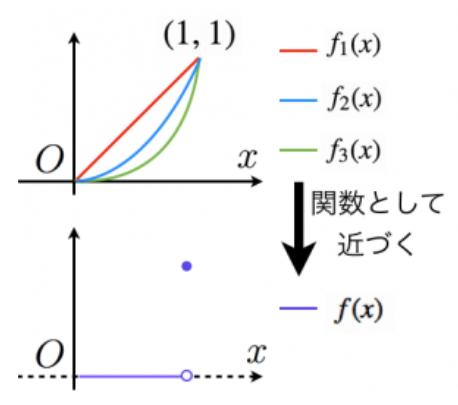
\includegraphics[clip,width=5cm]{./not_uni_conv.png}
        \caption{一様収束でない例}
        \end{center}
    \end{figure}

    \item[\bf{Theorem:}] 一様収束と連続性(関数級数version) \\
        距離空間$X, Y$に対し, 関数級数$\sum f_n,\ f_n : X \mapsto Y$が$X$において$s : X \mapsto Y$に一様収束するとき, 
        \begin{center}
        $f_n$が$x_* \in X$で連続 $\Rightarrow$ $\sum_{n=0}^k f_n$が$x_* \in X$で連続 $\Rightarrow$ $s = \sum f_n$が$x_* \in X$で連続 \end{center}
    
    \item[\bf{Theorem:}] 一様収束とリーマン積分. \\
        \point 一様収束前後でリーマン可積分の性質が保たれる.積分と極限の交換としても見れる. \\
        コンパクトな区間$I$上の関数列$(f_n),\ f_n : I \mapsto \mathbb{R}$が$I$において$f : I \mapsto \mathbb{R}$に一様収束するとき, 
        \begin{center} $f_n$が$I$でリーマン可積分 $\Rightarrow$ $f$が$I$でリーマン可積分. \end{center}
        $I=[a,\ b]$とすれば, 
        $$ \lim_{n \to \infty} \int_a^b f_n(x) dx \underset{一様収束}{=} \int_a^b f(x) dx = \int_a^b \lim_{n \to \infty} f_n(x) dx$$
        \begin{proof}
            $ | f_n(x) - f(x) | < \epsilon \Leftrightarrow f_n(x) - \epsilon < f(x) < f_n(x) + \epsilon$ \\ 
            $ \displaystyle \Rightarrow \underline{ \int_a^b} f_n(x) dx - \epsilon \leq \underline{ \int_a^b} f(x) dx  \leq \overline{ \int_a^b } f(x) dx  \leq \overline{ \int_a^b } f_n(x) dx + \epsilon $
        \end{proof} \\

    \item[\bf{Example:}] 一様収束でなく, 極限関数$f$がリーマン非可積分となる例.
        $$ f_n(x) = \lim_{m \to \infty} ( \cos n!\pi x )^{2m} \to f(x) = \begin{cases} \ 1 \quad \text{(xが有理数)} \\ \ 0 \quad \text{(xが無理数)} \end{cases} $$
        $f_n$はリーマン可積分で, $\displaystyle \int_0^1 f_n(x) dx = 0$, $f$はリーマン非可積分.

    \item[\bf{Theorem:}] 項別積分の定理 \\
        \point 有限個の項なら自明.無限個の項でも成り立つことが本質. \\
        コンパクトな区間$I$上の関数級数$\sum f_n,\ f_n : I \mapsto \mathbb{R}$が$I$において$s :I \mapsto \mathbb{R}$に一様収束するとき, 
        \begin{center} $f_n$が$I$でリーマン可積分 $\Rightarrow$ $\sum_{n=1}^m f_n$が$I$でリーマン可積分. $\Rightarrow$ $s = \sum f_n$が$I$でリーマン可積分. \end{center}
        $I=[a,\ b]$とすれば, 
        $$ \int_a^b( \sum_{n=0}^{\infty} f_n(x)) dx = \sum_{n=0}^{\infty} \int_a^b f_n(x) dx$$
        \begin{proof}
            $ \displaystyle \int_a^b \lim_{n \to \infty} \sum_{k=0}^n f_k(x) dx \underset{一様収束}{=} \lim_{n \to \infty} \int_a^b \sum_{k=0}^n f_k(x) dx \underset{有限和の交換}{=} \lim_{n \to \infty} \sum_{k=0}^n \int_a^b f_k(x) dx$
        \end{proof}

    \item[\bf{Example:}] 項別積分の定理の成立例
        $$ \cos x = \sum_{n=0}^{\infty} \frac{\cos^{(n)}(0)}{n!} x^n = 1 - \frac{x^2}{2!} + \frac{x^4}{4!} - \frac{x^6}{6!} + \cdots $$
        $\displaystyle \sum_{n=0}^{\infty} \frac{\cos^{(n)}(0)}{n!} x^n$は整級数.比判定法を用いれば$\beta = \displaystyle \limsup_{n \to \infty} \dfrac{1}{n+1} = 0$より, 収束半径$R = \infty$. \\
        整級数は$\{ x \mid 0 < |x| < \infty\}$においてコンパクト一様収束する.よって, 項別積分の定理が使える.
        \begin{eqnarray*}
            \int_a^b \cos x dx &=& \int_a^b \sum_{n=0}^{\infty} \frac{\cos^{(n)}(0)}{n!} x^n dx \underset{項別積分}{=} \sum_{n=0}^\infty \int_a^b \frac{\cos^{(n)}(0)}{n!} x^n dx \\ 
            &=&\sum_{n=0}^{\infty} \frac{\sin^{(n+1)}(0)}{(n+1)!} x^{n+1} = \sin x
        \end{eqnarray*}

    \item[\bf{Theorem:}] 一様収束と微分 \\
        \point : $f_n$の一様収束性だけでは微分可能性は移せない. \\
        区間$I$上の関数列$(f_n),\ f_n : I \mapsto \mathbb{R}$が以下の条件を満たすとき, 
        \begin{itemize}
            \item $f_n$は区間$I$上で微分可能.
            \item ある1点$x_* \in I$において, $(f_n)$が$f$に各点収束.
            \item 関数列$(f'_n)$は区間$I$上でコンパクト一様収束.
        \end{itemize}
        \begin{center} 
            $f_n$が$I$上で微分可能 $\Rightarrow$ $f_n$は$I$上で$f$にコンパクト一様収束, $f$が$I$上で微分可能.
        \end{center}
        $$\lim_{n \to \infty} \frac{\mathrm{d}}{\mathrm{d} x} f_n(x) \underset{f_n'の一様収束}{=} \frac{\mathrm{d}}{\mathrm{d} x} \lim_{n \to \infty} f_n(x) = \frac{\mathrm{d}}{\mathrm{d} x} f(x)$$
        \begin{proof}
            
        \end{proof}
    
    \item[\bf{Theorem:}] 項別微分の定理 \\
        \point 有限個の項なら自明.無限個の項でも成り立つことが本質. \\
        区間$I$上の関数級数$\sum f_n,\ f_n : I \mapsto \mathbb{R}$が以下の条件を満たすとき, 
        \begin{itemize}
            \item $f_n$は区間$I$上で微分可能.
            \item ある1点$x_* \in I$において, $\sum f_n$が$s$に各点収束.
            \item 関数列$(\sum f_n)' = \sum f_n'$は区間$I$上でコンパクト一様収束.
        \end{itemize}
        \begin{center}
            $f_n$が$I$上で微分可能 $\Rightarrow$ $\sum_{n=1}^m f_n$が$I$上で微分可能 $\Rightarrow$ $s = \sum f_n$が$I$上で微分可能.
        \end{center}
        $$ \frac{\mathrm{d}}{\mathrm{d} x} \sum_{n=1}^{\infty} f_n(x) = \sum_{n=1}^{\infty} \frac{\mathrm{d}}{\mathrm{d} x} f_n(x)$$
        \begin{proof}
            $ { \displaystyle \dfrac{\mathrm{d}}{\mathrm{d} x} \lim_{n \to \infty} \sum_{k=1}^n f_k(x) \underset{\sum f_k'の一様収束}{=} \lim_{n \to \infty} \dfrac{\mathrm{d}}{\mathrm{d} x} \sum_{k=1}^{n} f_k(x) \underset{有限和の交換}{=} \lim_{n \to \infty} \sum_{k=1}^{n} \dfrac{\mathrm{d}}{\mathrm{d} x} f_k(x) = \sum_{n=1}^{\infty} \frac{\mathrm{d}}{\mathrm{d} x} f_n(x) }$
        \end{proof}
        
        
\end{description}

\section{級数}
\begin{description}
    \item[\bf{Definition:}] 数列$(a_n)$に定められる(無限)級数
        $$ s_{\infty} = \sum a_n = \sum_{n=0}^{\infty} a_n $$
        ただし, 部分和の数列$(s_n)$以下のように定められる.
        $$(s_n) =  \sum_{n=0}^{n} a_n$$
        
    \item[\bf{Definition:}] 級数の収束
        \begin{enumerate}
            \item 一定値$s$に収束. \\
                級数の和$\displaystyle s=\sum_{n=0}^{\infty} a_n$が存在. $\Leftrightarrow (s_n)\text{がCauchy列}$

            \item 発散 \\
                $\displaystyle \sum_{n=0}^{\infty} a_n = + \infty$ または $\displaystyle \sum_{n=0}^{\infty} a_n = - \infty$ 
        \end{enumerate}

    \item[\bf{Theorem:}] 級数の演算 \\
        級数$\sum a_n,\ \sum b_n$が収束し, 和$a,\ b$を持つ. $\Rightarrow$
        $$\begin{cases} \ \sum \left( a_{n}+b_{n}\right) =a+b \\ \ \sum ca_{n}=ca \quad (c : \text{定数})\end{cases}$$

    \item[\bf{Theorem:}] 級数が収束 $\Rightarrow \displaystyle \lim_{n \to \infty} a_n = 0$ \\
        \begin{proof}
            級数が収束 $\Rightarrow \displaystyle {|\sum_{k=n}^m a_k|} < \epsilon$, $m=n$とすれば$a_n \rightarrow 0 \ (n \to \infty)$の定義そのもの.
        \end{proof}

    \item[\bf{Theorem:}] 級数が絶対収束 $\Rightarrow$ 級数は収束. \\
        $$ \begin{cases}
            \ \sum a_n \text{が絶対収束} \overset{\mathrm{def}}{\Leftrightarrow} \text{級数}\sum |a_n|\text{が収束.} \\
            \ \sum a_n \text{が条件収束} \overset{\mathrm{def}}{\Leftrightarrow} \text{絶対収束しないが, }\sum a_n\text{は収束.}
        \end{cases} $$
        \begin{proof}
            $\displaystyle |\sum_{k=n}^m a_k| \leq \sum_{k=n}^m |a_k| < \epsilon$より, $(s_n)$がCauchy列.
        \end{proof} \\
        \point 絶対収束すると良いこと : 順序変更が可能.(配列替え級数)
    
    \item[\bf{Theorem:}] 級数$\sum a_n$が絶対収束 $\Rightarrow \sum a_n$の任意の配列がえ級数も絶対収束.同じ収束値をもつ.
        
    \item[\bf{Theorem:}] 根判定法(root Test) \\
        級数$\sum a_n$において, 
        $$\limsup_{n \to \infty} \sqrt[n]{|a_n|} = \alpha$$
        $$ \begin{cases} \ \alpha < 1 \Rightarrow \sum a_{n} \text{は絶対収束} \\ 
        \ \alpha > 1 \Rightarrow \sum a_{n} \text{は発散} \end{cases} $$
    
    \item[\bf{Example:}] 等比級数の収束判定 \\
        級数$\sum a_n,\ a_n = r^n $に対して適用.
        $$ \limsup_{n \to \infty} \sqrt[n]{|a_n|} = r $$
        $$\begin{cases} \ r < 1 \Rightarrow \sum a_{n} \text{は絶対収束} \\ 
        \ r > 1 \Rightarrow \sum a_{n} \text{は発散} \end{cases} $$
        収束するとき
        $$ \sum_{n=0}^{\infty} a_n = \frac{1}{1-r}$$
        
    \item[\bf{Theorem:}] 比判定法(ratio Test) \\
        級数$\sum a_n$において, 
        $$ \limsup_{n \to \infty} |\frac{a_{n+1}}{a_n}| = \alpha $$
        $$ \begin{cases} \ \alpha < 1 \Rightarrow \sum a_{n} \text{は絶対収束} \\
            \ \alpha \geq 1 \Rightarrow \sum a_{n} \text{は発散} \end{cases} $$

    \item[\bf{Example:}] $\displaystyle \sum_{n=1}^{\infty} \frac{1}{2n-1}$の収束判定 
        \begin{eqnarray*}
            \limsup_{n \to \infty} |\frac{a_{n+1}}{a_n}| &=& \limsup_{n \to \infty} |\frac{2n-1}{2(n+1)-1}| = 1
        \end{eqnarray*}

    \item[\bf{Theorem:}] 根判定法と比判定法の比較
        $$ \begin{cases} \ \displaystyle { \liminf_{n \to \infty}  \frac{a_{n+1}}{a_n} \leq \liminf_{n \to \infty} \sqrt[n]{a_n} } \\ 
        \ \displaystyle { \limsup_{n \to \infty} \sqrt[n]{a_n} \leq \liminf_{n \to \infty} \frac{a_{n+1}}{a_n} } \end{cases} $$
    \point 比判定法は計算が簡便.判定の有効性は根判定法の方が高い.

    
    \item[\bf{Theorem:}] オイラーマクローリンの判定法 \\
        (追記予定)
\end{description}
    \subsection{正項級数}
    \begin{description}
        \item[\bf{Definition:}] 正項級数$\sum a_n \overset{\mathrm{def}}{\Leftrightarrow} \forall n \in \mathbb{N},\ a_n \geq 0 $ \\
            部分和の数列$(s_n)$は単調増加数列となる.

        \item[\bf{Example:}] 正項級数の例 \\
            $$ \sum_{n=0}^{\infty} \frac{1}{n!} = 1 + \frac{1}{1!} + \frac{1}{2!} + \cdots $$ 

        \item[\bf{Theorem:}] 正項級数$\sum a_n$が収束 $\Leftrightarrow$
            $$ \text{部分和数列} (s_n) \text{が上に有界} \Leftrightarrow \exists M \in \mathbb{R},\ s_n \geq M$$
        
        \item[\bf{Theorem:}] 比較定理(正項級数の収束判定) \\
            正項級数$\sum a_n,\ \sum b_n$に対し, $\forall n, a_n \leq k b_n \quad (k > 0)$が成立するとき, 
            \begin{enumerate}
                \item $\sum b_n$が収束 $\Rightarrow$ $\sum a_n$は収束
                \item $\sum a_n$が発散 $\Rightarrow$ $\sum b_n$は発散
            \end{enumerate}
        
        \item[\bf{Example:}] 比較定理を使った収束判定
            
    \end{description}

    \subsection{整級数(べき級数)}
    \begin{description}
        \item[\bf{Definition:}] 正級数$\sum a_n$\\
            $$ \sum a_n = \sum_{n=0}^{\infty} b_n x^n = b_0 + b_1x + b_2x^2 + \cdots $$

        \item[\bf{Theorem:}] 収束半径$R$ \\
            整級数$\sum b_nx^n$において,
            $$\beta =\limsup_{n \to \infty} \sqrt[n]{|b_n|} \ \text{または} \ \beta =\limsup_{n \to \infty} |\frac{b_{n+1}}{b_n}|,\ R = \frac{1}{\beta}$$
            $$\begin{cases} \ \beta|x| < 1 \Leftrightarrow |x| < R \Rightarrow \sum b_nx^n \text{は絶対収束かつコンパクト一様収束} \\ 
            \ \beta|x| > 1 \Leftrightarrow |x| > R \Rightarrow \sum b_{n}x^n \text{は発散} \end{cases} $$

        \item[\bf{Example:}] 有名なテイラー展開の収束半径 \\
    
    \end{description}
    \subsection{複素級数}
\section{微分}
        \begin{description}
            \item[\bf{Definition}] $f: X \mapsto Y$の$x=x_0$における微分可能性
                \begin{itemize}
                    \item $X \underset{open}{\subseteq} \mathbb{R},\ Y = \mathbb{R}$ (1変数実数値関数)
                        $$ \lim_{h \to 0} \dfrac{f(x_0 + h) - f(x_0) - f'(x_0)h }{h} = 0 \text{を満たす定数} f'(x_0) \text{が存在}$$
                        別表現では, 
                        $$f(x_0 + h) - f(x_0) = f'(x_0)h + o(h),\ \displaystyle \lim_{h \to 0} \dfrac{o(h)}{h} = 0 \text{を満たす定数} f'(x_0) \text{が存在.}$$
                        
                    \item $X \underset{open}{\subseteq} \mathbb{R}^n,\ Y = \mathbb{R}$ (多変数実数値関数)
                        $$ \lim_{||\bm{h}|| \to 0} \dfrac{f(\bm{x_0} + \bm{h}) - f(\bm{x_0}) - \bm{f'}(\bm{x_0}) \cdot \bm{h} }{||\bm{h}||} = 0 \text{を満たす定数} \bm{f'}(\bm{x_0}) \text{が存在}$$
                        別表現では, 
                        $$f(\bm{x_0} + \bm{h}) - f(\bm{x_0}) = \bm{f'}(\bm{x_0}) \cdot \bm{h} + o(||\bm{h}||),\ \displaystyle \lim_{||\bm{h}|| \to 0} \dfrac{o(||\bm{h}||)}{||\bm{h}||} = 0 \text{を満たす定数} \bm{f'}(\bm{x_0}) \text{が存在.}$$
                        $\bm{f'}(\bm{x_0})$ は勾配ベクトルと呼ばれる.
                        $$\bm{f'}(\bm{x_0}) = (\mathrm{grad} \ f)(\bm{x_0}) = ( \frac{\partial f}{\partial x_1},\ \frac{\partial f}{\partial x_2},\ \dots  ,\ \frac{\partial f}{\partial x_n} )(\bm{x_0}) $$
                        $\bm{f'}(\bm{x_0}) \cdot \bm{h}$ は全微分と呼ばれる.
                        $$\bm{f'}(\bm{x_0}) \cdot \bm{h} = \frac{\partial f}{\partial x_1} \mathrm{d} x_1 + \frac{\partial f}{\partial x_2} \mathrm{d} x_2 + \dots + \frac{\partial f}{\partial x_n} \mathrm{d} x_n $$
                        
                    \item $X \underset{open}{\subseteq} \mathbb{R}^n,\ Y = \mathbb{R}^m$ (多変数ベクトル値関数)
                        $$ \lim_{\bm{||h||} \to 0} \dfrac{||\bm{f}(\bm{x_0} + \bm{h}) - \bm{f}(\bm{x_0}) - \bm{f'}(\bm{x_0}) \bm{h} ||}{||\bm{h}||} = 0 \text{を満たす定数} \bm{f'}(\bm{x_0}) \text{が存在.}$$
                        別表現では, 
                        $$\bm{f}(\bm{x_0} + \bm{h}) - \bm{f}(\bm{x_0}) = \bm{f'}(\bm{x_0}) \bm{h} + \bm{o}(||\bm{h}||),\ \lim_{||\bm{h}|| \to 0} \dfrac{||\bm{o}(||\bm{h}||)||}{||\bm{h}||} = 0 \text{を満たす定数} \bm{f'}(\bm{x_0}) \text{が存在.}$$
                        $\bm{f}$を座標関数を用いて表現すると, 
                        $$\begin{bmatrix}
                            f_1(\bm{x_0} + \bm{h}) \\
                            f_2(\bm{x_0} + \bm{h}) \\
                                \vdots \\
                            f_m(\bm{x_0 + \bm{h}})
                        \end{bmatrix}  
                        - 
                        \begin{bmatrix}
                            f_1(\bm{x_0}) \\
                            f_2(\bm{x_0}) \\
                                \vdots \\
                            f_m(\bm{x_0})
                        \end{bmatrix}
                        = 
                        \begin{bmatrix}
                            \mathrm{grad} \ f_1(\bm{x_0}) \\
                            \mathrm{grad} \ f_2(\bm{x_0}) \\
                                \vdots \\
                            \mathrm{grad} \ f_m(\bm{x_0})
                        \end{bmatrix}
                        \bm{h} + \bm{o}(||\bm{h}||),\ \lim_{||\bm{h}|| \to 0} \dfrac{||\bm{o}(||\bm{h}||)||}{||\bm{h}||} = 0 $$

                        $\bm{f'}(\bm{x_0})$ はヤコビ行列と呼ばれる.
                        $$\bm{f'}(\bm{x_0}) = \bm{J_f}(\bm{x_0}) = 
                        \begin{bmatrix}
                            \mathrm{grad} \ f_1(\bm{x_0}) \\
                            \mathrm{grad} \ f_2(\bm{x_0}) \\
                                \vdots \\
                            \mathrm{grad} \ f_m(\bm{x_0})
                        \end{bmatrix}
                        = 
                        \begin{bmatrix}
                            \frac{\partial f_1}{\partial x_1}(\bm{x_0}) & \cdots & \frac{\partial f_1}{\partial x_n}(\bm{x_0}) \\
                            \vdots & & \vdots \\
                            \frac{\partial f_m}{\partial x_1}(\bm{x_0}) & \cdots & \frac{\partial f_m}{\partial x_n}(\bm{x_0})
                        \end{bmatrix} \in M(m,n; \mathbb{R})$$
                \end{itemize}
        
        \item[\bf{Definition:}] 実数値関数$f : \mathbb{R}^n \mapsto \mathbb{R}$の偏微分係数 \\
            $$ \frac{\partial f}{\partial x_i}((x_1,\ x_2,\ \dots,\ x_n)) = \lim_{h \to 0} \dfrac{f(x_1,\ \dots ,\ x_i + h,\ \dots ,\ x_n) - f(x_1,\ \dots ,\ x_i,\ \dots ,\ x_n)}{h}$$

        \item[\bf{Definition:}] 実数値関数$f : \mathbb{R}^n \mapsto \mathbb{R}$のベクトル$\bm{v}$向きの方向微分 \\
            \point : 偏微分の一般化.偏微分は標準基底ベクトル向きの方向微分と捉えることができる.
            $$ (D_{\bm{v}}f)(\bm{x}) = \lim_{h \to 0} \dfrac{f(\bm{x} + h\bm{v})-f(\bm{x})}{h||\bm{v}||}$$
            $\bm{v}$を正規化し, $\bm{u} = \frac{\bm{v}}{||\bm{v}||}$とした場合の式は, 
            $$ (D_{\bm{u}}f)(\bm{x}) = \lim_{h \to 0} \dfrac{f(\bm{x} + h\bm{u})-f(\bm{x})}{h}$$
            $\gamma : \mathbb{R} \mapsto \mathbb{R}^n,\ \gamma (t) = \bm{x} + t \bm{u}$を用いると, 
            $$ (D_{\bm{u}}f)(\bm{x}) = \frac{\mathrm{d} (f \circ \gamma)}{\mathrm{d} t}(0) \underset{微分鎖律}{=} (\mathrm{grad} \ f)(\bm{x}) \cdot \bm{u}$$
            \point 微分係数の大きさを最大にする方向は, $\mathrm{grad} \ f$であるとわかる.
    
        \item[\bf{Definition:}] $C^r$級の関数$f: X \mapsto Y$
            \begin{itemize}
                \item $X \underset{open}{\subseteq} \mathbb{R}^n,\ Y = \mathbb{R}$ (多変数実数値関数)
                    \begin{center} 
                        関数$f$が$C^r$級 $\defEq$ $r$次の偏導関数が全て存在し, 連続関数である. \\
                        特に, $C^1$級 $\defEq$ $\frac{\partial f}{\partial x_1},\ \frac{\partial f}{\partial x_2}, \dots,\ \frac{\partial f}{\partial x_n}$が存在し, 連続関数である.
                    \end{center}
                \item $X \underset{open}{\subseteq} \mathbb{R}^n,\ Y = \mathbb{R}^m$ (多変数ベクトル値関数)
                    \begin{center} 
                        関数$\bm{f}$が$C^r$級 $\defEq$ 座標関数$f_i$が全て$C^r$級
                    \end{center}
            \end{itemize}

        \item[\bf{Remark:}] $C^1$級, 微分可能性, 連続性の関係 \\
            $C^1$級 $\Leftrightarrow$ 連続的微分可能 $\Leftrightarrow$ $1$次の偏導関数が全て存在$\wedge$偏導関数が全て連続. \\
            $C^1$級 $\Rightarrow$ 微分可能 $\Rightarrow$ $1$次の偏導関数が全て存在, $f$が連続.
        
        \item[\bf{Example:}] 偏微分係数は存在するが, 微分可能でない例 \\
        \item[\bf{Theorem:}] 微分鎖律
            \begin{itemize}
                \item $U \underset{open}{\subseteq} \mathbb{R},\ g : U  \mapsto \mathbb{R}^n,\ g(U) \underset{open}{\subseteq} V,\ f : V \mapsto \mathbb{R},\ f \circ g : U \mapsto \mathbb{R}$ (多変数実数値関数)
                    \begin{eqnarray*}
                        \dfrac{\partial (f \circ g)}{\partial t}(t_0) &=& (\mathrm{grad} \ f)(g(t_0)) \cdot \dfrac{\partial g}{\partial t}(t_0) \\
                            &=& ( \frac{\partial f}{\partial x_1}(g(t_0)),\ \frac{\partial f}{\partial x_2}(g(t_0)),\ \dots  ,\ \frac{\partial f}{\partial x_n}(g(t_0)) ) \cdot (\frac{\partial x_1}{\partial t}(t_0),\ \frac{\partial x_2}{\partial t}(t_0),\ \dots  ,\ \frac{\partial x_n}{\partial t}(t_0)) \\
                            &=& (\sum_{i=1}^n \frac{\partial f}{\partial x_i} \frac{\partial x_i}{\partial t})(t_0)
                    \end{eqnarray*}
                
                    \begin{proof}
                        $f(\bm{x}+\bm{k}) - f(\bm{x}) = f(\bm{g}(t + h)) - f(\bm{g}(t)) = (\mathrm{grad} \ f) \cdot (\bm{g}(t+h)-\bm{g}(t)) + o(||\bm{k}||) $
                    \end{proof}
                    
                \item $U \underset{open}{\subseteq} \mathbb{R}^l,\ g : U  \mapsto \mathbb{R}^n,\ g(U) \underset{open}{\subseteq} V,\ f : V \mapsto \mathbb{R}^m,\ f \circ g : U \mapsto \mathbb{R}^m$ (多変数ベクトル値関数)
                    \begin{eqnarray*}
                        \dfrac{\partial (\bm{f \circ g})}{\partial \bm{t}}(\bm{t_0}) &=& \bm{J_f}(\bm{g}(\bm{t_0})) \bm{J_g}(\bm{t_0}) \ ( \bm{J_f}(\bm{g}(\bm{t_0})) \in M(m,n;\mathbb{R}),\ \bm{J_g}(\bm{t_0}) \in M(n,l) )\\
                            &=& \begin{bmatrix}
                                \frac{\partial f_1}{\partial x_1}(\bm{g}(\bm{t_0})) & \cdots & \frac{\partial f_1}{\partial x_n}(\bm{g}(\bm{t_0}))\\
                                \vdots & & \vdots \\
                                \frac{\partial f_m}{\partial x_1}(\bm{g}(\bm{t_0})) & \cdots & \frac{\partial f_m}{\partial x_n}(\bm{g}(\bm{t_0}))
                            \end{bmatrix} \begin{bmatrix}
                                \frac{\partial x_1}{\partial t_1}(\bm{t_0}) & \cdots & \frac{\partial x_1}{\partial t_l}(\bm{t_0}) \\
                                \vdots & & \vdots \\
                                \frac{\partial x_n}{\partial t_1}(\bm{t_0}) & \cdots & \frac{\partial x_n}{\partial t_l}(\bm{t_0})
                            \end{bmatrix} \\
                            &=& \begin{bmatrix}
                                (\sum_{i=1}^n \frac{\partial f_1}{\partial x_i} \frac{\partial x_i}{\partial t_1})(\bm{t_0}) & \cdots & (\sum_{i=1}^n \frac{\partial f_1}{\partial x_i} \frac{\partial x_i}{\partial t_l})(\bm{t_0}) \\
                                \vdots & & \vdots \\
                                (\sum_{i=1}^n \frac{\partial f_m}{\partial x_i} \frac{\partial x_i}{\partial t_1})(\bm{t_0}) & \cdots & (\sum_{i=1}^n \frac{\partial f_m}{\partial x_i} \frac{\partial x_i}{\partial t_l})(\bm{t_0})
                            \end{bmatrix} \in M(m,l;\mathbb{R})
                    \end{eqnarray*}
            \end{itemize}

        \item[\bf{Theorem:}] 微分演算子の順序交換
        \item[\bf{Example:}] 微分演算子の順序が交換できない例: p161:1
        \end{description}


\section{ロルの定理, 平均値の定理, テイラーの定理}
\begin{description}
    \item[\bf{Theorem:}] ロルの定理
        $$ f: [a,\ b] \mapsto \mathbb{R},\ [a,\ b] \text{で連続},\ (a,\ b) \text{で微分可能},\ f(a) = f(b) \Rightarrow \exists c \in (a,\ b) : f'(c) = 0$$
        \proof $f([a,\ b])$はコンパクトより, 最大最小値をもつ.最大値の点では右微分係数$\leq 0$, 左微分係数$\geq 0$ \\
        \point ロルの定理を使うときは, おもむろに$g(a) = g(b)$となるような関数$g$を定義することが多い.
    \item[\bf{Theorem:}] 平均値の定理
        \begin{itemize}
            \item ラグランジュの平均値の定理 \\
            $$ f: [a,\ b] \mapsto \mathbb{R},\ [a,\ b] \text{で連続},\ (a,\ b) \text{で微分可能} \Rightarrow \exists c \in (a,\ b) : \dfrac{f(b) - f(a)}{b - a} = f'(c)$$
            \proof $h(x) = f(x) + Cx$を定義し, $h(a)=h(b)$を満たすように$C$を定める.
            \item コーシーの平均値の定理 \\
            $ f,\ g: [a,\ b] \mapsto \mathbb{R},\ [a,\ b] \text{で連続},\ (a,\ b) \text{で微分可能},\ \forall x \in (a,\ b) : g'(x) \neq 0$
            $$ \Rightarrow \exists c \in (a,\ b) : \dfrac{f(b) - f(a)}{g(b) - g(a)} = \dfrac{f'(c)}{g'(c)}$$
            \proof $h(x) = f(x) + Cg(x)$を定義し, $h(a)=h(b)$を満たすように$C$を定める. \\
            \point ラグランジュの平均値の定理の一般化.
        \end{itemize}
    \item[\bf{Theorem:}] ロピタルの定理 \\
        $f,\ g: (a,\ b) \mapsto \mathbb{R},\ (a,\ b) \text{で微分可能},\ \forall x \in (a,\ b) : g'(x) \neq 0,\ { \color{red} \displaystyle \lim_{x \to a} \dfrac{f'(x)}{g'(x)} = A \in \mathbb{R} \cup \{ +\infty,\ -\infty \} }$ 
        \begin{itemize}
            \item $\dfrac{0}{0}$の不定形
                $$\lim_{x \to a} f(x) = 0,\ \lim_{x \to a} g(x) = 0 \Rightarrow \lim_{x \to a} \dfrac{f(x)}{g(x)} = \lim_{x \to a} \dfrac{f'(x)}{g'(x)} = A$$
            \item $\dfrac{\infty}{\infty}$の不定形
                $$\lim_{x \to a} g(x) = \pm \infty \Rightarrow \lim_{x \to a} \dfrac{f(x)}{g(x)} = \lim_{x \to a} \dfrac{f'(x)}{g'(x)} = A$$
        \end{itemize}
    \item[\bf{Theorem:}] テイラーの定理, 関数$f : X \mapsto Y$の近似多項式. \\
        \point $f(x) \ (x \in X)$の値を$a \in X$から多項式で近似する. $n = 1$で打ち切ると平均値の定理.
        \begin{itemize}
            \item $X = [a,\ b] \subseteq \mathbb{R},\ Y = \mathbb{R}$, $f$は$[a,\ b]$上で連続, $(a,\ b)$上でn回微分可能. 
                $$ f(x) = \sum_{k = 0}^{n-1} \dfrac{f^{(k)}(a)}{k!}(x-a)^k + R_n,\ R_n = \dfrac{f^{(n)}(c)}{n!}(x-a)^n,\ c \in (a,\ x) $$
                \begin{proof} 証明の方針 : $R_n = \dfrac{C}{n!}(x-a)^n$とした時に, $C = f^{(n)}(c)$となる$c$の存在を示す.
                    \begin{enumerate}
                        \item $g(x) = f(b) - \displaystyle \sum_{k = 0}^{n-1} \dfrac{f^{(k)}(x)}{k!}(b-x)^k - \dfrac{C}{n!}(b-x)^n$を定義.
                        \item $g(a) = g(b) = 0$より, ロルの定理から$\exists c \in [a,\ b] : g'(c) = 0$
                        \item $g'(x) = (C - f^{(n)}(x))\dfrac{(b-x)^{n-1}}{(n-1)!}$ より, $g'(c) \Rightarrow C = f^{(n)}(c)$      
                    \end{enumerate}
                \end{proof}

            \item $X \underset{open}{\subseteq} \mathbb{R}^n,\ Y = \mathbb{R}$, $f$は$X$で$C^r$級.
                $$ f(\bm{x}) = \sum_{k=0}^{n-1} \dfrac{( (\bm{x} - \bm{a}) \cdot \mathrm{grad})^k f}{k!}(\bm{a}) + R_n,\ R_n = \dfrac{( (\bm{x} - \bm{a}) \cdot \mathrm{\mathrm{grad}})^n f}{n!}(\bm{a}+ \theta (\bm{x} - \bm{a})),\ 0 < \theta < 1$$
                \point : $( (\bm{x} - \bm{a}) \cdot \mathrm{\mathrm{grad}})$ はスカラーの微分演算子となっている. \\
                \begin{proof} 証明の方針 : $g(t) = f(\bm{a} + t(\bm{x} - \bm{a}))$を定義し, $t=0$周りの1変数テイラー展開を行う.
                    \begin{enumerate}
                        \item $\dfrac{\partial g}{\partial t}(t_0) = (\mathrm{grad} \ f)(g(t_0)) \cdot (\bm{x} - \bm{a}) = ((\bm{x} - \bm{a}) \cdot \mathrm{grad})(f(g(t_0)))$
                        \item $t=0$周りでのテイラー展開$g(t) = \displaystyle \sum_{k = 0}^{n-1} \dfrac{g^{(k)}(0)}{k!}(t)^k + R_n$
                        \item $t=1$を代入. $g(1) = \displaystyle \sum_{k = 0}^{n-1} \dfrac{g^{(k)}(0)}{k!} + R_n = \displaystyle \sum_{k = 0}^{n-1} \dfrac{( (\bm{x} - \bm{a}) \cdot \mathrm{grad})^k f}{k!}(\bm{a}) + R_n$
                    \end{enumerate}
                \end{proof}
        \end{itemize}
    
    \item[\bf{Theorem:}] 誤差項$R_n$の評価 \\
        $\bm{a}$周りでの$r$次までのテイラー展開式を$P_r(\bm{x}; \bm{a})$とする.
            $$ P_r(\bm{x}; \bm{a}) = f(\bm{a}) + \dfrac{( (\bm{x} - \bm{a}) \cdot \mathrm{\mathrm{grad}})}{1!}f(\bm{a}) + \cdots + \dfrac{( (\bm{x} - \bm{a}) \cdot \mathrm{\mathrm{grad}})^r}{r!}f(\bm{a}) $$
        誤差項$R_{r+1}$は, 
        $$ R_{r+1}(\bm{x},\ \bm{a}) = f(\bm{x}) - P_r(\bm{x}; \bm{a}),\ \lim_{||(\bm{x} - \bm{a})|| \to 0}  \dfrac{ R_{r+1}(\bm{x},\ \bm{a})}{||(\bm{x} - \bm{a})||^r} = 0$$
        \point $\bm{x}$が$\bm{a}$に近づくスピードより速く近似多項式$P$は元の関数$f$に近づく.
\end{description}

\section{逆写像定理, 陰関数定理}
\begin{description}
    \item[\bf{Theorem:}] 逆写像定理 \\
        \point : $f$の微分が死んでいない点の近傍では, $f$には逆写像が存在し, 逆写像の微分も可能. \\
        $C^1$級写像$\bm{f} : U \opensubset \mathbb{R}^n \mapsto \mathbb{R}^n$が, 
        $\bm{a} \in U$においてヤコビ行列$\bm{f}'(\bm{a})$が正則のとき,
        $$ \bm{a} \text{の近傍} U_0 \opensubset U \text{で} \bm{f} : U_0 \mapsto V_0 \opensubset \mathbb{R} \ \text{は可逆(全単射)} ,\ \bm{f}^{-1} \text{も} C^1 \text{級写像}$$
        ただし, ヤコビ行列$\bm{f}'(\bm{a})$は
        $$ \bm{f}'(\bm{a}) = \begin{bmatrix}
            \frac{\partial f_1}{\partial x_1}(\bm{a}) & \cdots & \frac{\partial f_1}{\partial x_n}(\bm{a}) \\
            \vdots & & \vdots \\
            \frac{\partial f_n}{\partial x_1}(\bm{a}) & \cdots & \frac{\partial f_n}{\partial x_n}(\bm{a})
        \end{bmatrix} \in M(n,n;\mathbb{R})$$
        $\bm{f}^{-1}$は以下のようにかける.
        $$ ({\bm{f}^{-1}})'(\bm{y}) = (\bm{f}'(\bm{x}))^{-1},\ \bm{y} = \bm{f}(\bm{x}) $$
    
        \begin{proof} 証明のステップ.
            \begin{enumerate}
                \item $\bm{f}$が$U_0$上で単射.
                \item $V_0 = \bm{f}(U_0)$が開集合.
                \item $f^{-1} : V_0 \mapsto U_0$が$V_0$上で微分可能かつ$({\bm{f}^{-1}})'(\bm{y}) = (\bm{f}'(\bm{x}))^{-1}$
                \item $(\bm{f}^{-1})'$が$V_0$上で連続.
            \end{enumerate}
        \end{proof}
    
    \item[\bf{Theorem:}] 陰関数定理 \\
        $C^1$級写像$\bm{f} : U \opensubset \mathbb{R}^{n+m} \mapsto \mathbb{R}^n$が, $(\bm{a},\ \bm{b}) \in U$において$\bm{f}(\bm{a},\bm{b}) = \bm{0}$かつ, \\
        ヤコビ行列$\bm{f}'((\bm{a}, \bm{b})) = \bm{f}'((\bm{a}, \bm{0})) + \bm{f}'((\bm{0}, \bm{b})) = \bm{f}_x'(\bm{a}) + \bm{f}_y'(\bm{b})$に対し$\bm{f}_x'(\bm{a})$が正則のとき, 
        
        $$\exists U_0 \opensubset U,\ \exists W_0 \opensubset \mathbb{R}^m$$
        \begin{eqnarray*}
            \forall \bm{y} \in W_0,\ (\bm{x},\ \bm{y}) \in U_0,\ \exists_1 \bm{x} \in \mathbb{R}^n : \bm{f}(\bm{x},\ \bm{y}) = 0 \\
            \Leftrightarrow \exists_1 \bm{g} : (\bm{g} : W_0 \mapsto \mathbb{R}^n),\ \bm{g}(\bm{b}) = a,\ \bm{f}(\bm{g}(\bm{y}),\ \bm{y}) = \bm{0}
        \end{eqnarray*}
        さらに, $\bm{g}$は$C^1$級写像であり, 
        $$ \forall y \in W_0,\ \bm{x} = \bm{g}(\bm{y}),\ \bm{g}'(\bm{y}) = - \bm{f}'_x(\bm{x})^{-1} \bm{f}'_y(\bm{y}) $$

        \begin{proof} 証明
            \begin{enumerate}
                \item $\bm{F} : U \mapsto \mathbb{R}^{n+m}, F(\bm{x},\ \bm{y}) = ( f(\bm{x}, \bm{y}), \bm{y})$を定義.ヤコビ行列$F'$が$(\bm{a},\bm{b})$で正則であることを示す.
                \item 逆写像定理より, $(\bm{a},\ \bm{b})$の近傍$U_0$で$f$は全単射かつ微分可能. \\
                逆に$V_0 = \{ (\bm{x},\bm{y}) \mid \bm{x} = \bm{0} \}$をとって, $U_0 = F^{-1}(V_0)$とすれば$C^1$級$g(\bm{y}) = \bm{x}$が定義できる.
                \item %$(\frac{\partial }{\partial \bm{y}}\bm{f}(( \bm{g}(\bm{y}),\bm{y} )))(\bm{y_0}) = \bm{0} \Leftrightarrow \bm{f}'(( \bm{g}(\bm{y}),\bm{y} ))(\bm{g}'(\bm{y}),\bm{})  = \bm{0}$ 
            \end{enumerate}
        \end{proof}
    
    \item[\bf{Example:}]  
    \item[\bf{Theorem:}] ラグランジュ未定乗数法 \\
        $C^1$級写像$f,\ \phi : U \opensubset \mathbb{R}^n \mapsto \mathbb{R}$が, $\phi(\bm{x}) = 0$制約下で
        $$\bm{a} \in U \text{が} f \text{の極値点かつ}  \mathrm{grad} \ \phi(\bm{a}) \neq 0 \Rightarrow \exists \lambda \in \mathbb{R},\ \mathrm{grad} \ f(\bm{a}) = \lambda \ \mathrm{grad} \ \phi(\bm{a})$$
        \begin{proof} 証明の方針 : 陰関数定理を使う.
            \begin{enumerate}
                \item $\bm{a} \in U$が$\phi(\bm{a}) = 0,\ \mathrm{grad} \ f(\bm{a}) \neq 0$を満たす.$D_1 f(\bm{a}) \neq 0$なら陰関数定理より, \\
                $x_1 = g(x_2,\ x_3, \dots,\ x_n)$を満たす$g$が存在.$\tilde{\bm{x}} = ( x_2,\ x_3, \dots,\ x_n )$と表記する.
                \item $F(\tilde{\bm{x}}) = f(g(x_2,\ x_3, \dots,\ x_n), x_2, \dots,\ x_n)$を定義.$\mathrm{grad} \ f(\bm{a}) = 0$より \\
                $\mathrm{grad} \ F(\tilde{\bm{a}}) = \begin{bmatrix}
                    D_2 F(\tilde{\bm{a}}) \\
                    \vdots \\
                    D_{n-1} F(\tilde{\bm{a}}) 
                \end{bmatrix} = 
                \begin{bmatrix}
                    D_2 f(\bm{a}) + D_n f(\bm{a}) D_2g(\tilde{\bm{x}}) \\
                    \vdots \\
                    D_{n-1} f(\bm{a}) + D_n f(\bm{a}) D_{n-1}g(\tilde{\bm{x}})
                \end{bmatrix}
                $
                \item 陰関数定理より, $D_ig(\tilde{\bm{a}}) = -(D_1 \phi(\bm{a}))^{-1}(D_i \phi(\bm{a}))$を代入して, $\lambda = (D_1 \phi(\bm{a}))^{-1}(D_1 f(\bm{a}))$
            \end{enumerate}
        \end{proof}
        これを用いて, 
        $$ 
        \begin{cases} 
            \ \phi(\bm{a}) = \bm{0} \\
            \ f(\bm{a}) = \lambda \ \mathrm{grad} \ \phi(\bm{a})
        \end{cases}
        $$
        を満たす極値点の候補$\bm{a}$を求めることができる. \\
        \point : あくまで$f$の極値点である必要条件.
    \item[\bf{Example:}]
\end{description}
\section{極値問題}
\begin{description}
    \item[\bf{Definition:}] 関数$f : U \underset{open}{\subset} \mathbb{R}^n \mapsto \mathbb{R}$の極値点
        \begin{itemize} 
            \item 極大点$\bm{a} \in U$
                $$ \exists V \underset{open}{\subseteq} U,\ \forall \bm{x} \in V,\ f(\bm{a}) \geq f(\bm{x}) $$
            \item 狭義の極大点$\bm{a} \in U$
                $$ \exists V \underset{open}{\subseteq} U,\ \forall \bm{x} \in V,\ f(\bm{a}) > f(\bm{x}) $$       
        \end{itemize}
        \point 近傍をとって, 凸な部分を作れたら極大点
    
    \item[\bf{Theorem:}] $\bm{a}$が極値点 $\Rightarrow \forall i : 1 \leq i \leq n,\ D_i(\bm{a}) = 0$ \\
        \point : 極値点 $\Rightarrow$ 臨界点, 逆は成り立たないことに注意. \\
        \begin{proof}
            $ g(t) = f(\bm{a} + t \bm{e_i}) $, $f$の極値問題を1変数$g$の極値問題に帰着.
        \end{proof}
    
    \item[\bf{Theorem:}] $U\underset{open}{\subset} \mathbb{R}^n$上$C^2$級関数$f : U \mapsto \mathbb{R}$の臨界点における点の分類方法 \\
        $\bm{a} \in U$が臨界点のとき, Hesse対称行列$H_f(\bm{a})$の正負によって点の分類を行う.
        $$ H_f(\bm{a}) = 
        \begin{bmatrix}
            \frac{\partial^2 f}{\partial x_1^2}(f(\bm{a})) & \frac{\partial^2 f}{\partial x_1 \partial x_2}(f(\bm{a})) & \cdots & \frac{\partial^2 f}{\partial x_1 \partial x_n}(f(\bm{a})) \\
            \frac{\partial^2 f}{\partial x_2 \partial x_1}(f(\bm{a})) & \frac{\partial^2 f}{\partial x_2^2}(f(\bm{a})) & \cdots & \frac{\partial^2 f}{\partial x_2 \partial x_n}(f(\bm{a})) \\
            \vdots & \vdots & \ddots & \vdots \\
            \frac{\partial^2 f}{\partial x_n \partial x_1}(f(\bm{a})) &  \frac{\partial^2 f}{\partial x_n x_2}(f(\bm{a})) & \cdots & \frac{\partial^2 f}{\partial x_n^2}(f(\bm{a}))
        \end{bmatrix} 
        $$
        \begin{itemize}
            \item $H_f(\bm{a})$が負 $\Rightarrow$ $\bm{a}$は狭義の極大点
            \item $H_f(\bm{a})$が正 $\Rightarrow$ $\bm{a}$は狭義の極小点
            \item $H_f(\bm{a})$が不定符号 $\Rightarrow$ $\bm{a}$は極値点ではない.(鞍点)
        \end{itemize}
        
        \begin{proof} $\bm{a}$が狭義の極小点になることの証明.
            \begin{enumerate}
                \item $f$のテイラー展開の2次の項$\dfrac{( (\bm{x} - \bm{a}) \cdot \mathrm{\mathrm{grad}})^2}{2!}f(\bm{a}) = \dfrac{1}{2}(\bm{x} - \bm{a})^T H_f(\bm{a}) (\bm{x} - \bm{a}) = Q_{H_f}((\bm{x} - \bm{a}))$
                \item $\bm{h} = (\bm{x} - \bm{a})$とおき, $f(\bm{a} + \bm{h}) - f(\bm{a}) = \dfrac{1}{2} Q_{H_f}(\bm{h}) + R_3(\bm{h}) > 0$を示す.
                \item $\dfrac{Q_{H_f}(\bm{h})}{||\bm{h}||^2}=Q_{H_f}(\dfrac{\bm{h}}{||\bm{h}||})$で, 定義域がコンパクト集合$\{ \bm{x} \in \mathbb{R}^n \mid ||\bm{x}|| = 1 \}$となる.
                最小値$\epsilon> 0$が存在. $|\dfrac{R_3(\bm{h})}{||\bm{h}||^2}|$は, 適切に$\delta$を選んで$\dfrac{\epsilon}{2}$より小さくできる.
                よって, $\dfrac{1}{2} \dfrac{Q_{H_f}(\bm{h})}{||\bm{h}||^2} + \dfrac{R_3(\bm{h})}{||\bm{h}||^2} > 0$
            \end{enumerate}
        \end{proof}
        \begin{proof} $\bm{a}$が極値点でない証明.
            
        \end{proof}
\end{description}

\section{リーマン積分}
    \subsection{リーマン積分の定義}
    \begin{description}
        \item[\bf{Definition:}] 有界閉区間$I = [a,\ b]$の分割$\Delta$ \\
            $I$に対する数列$\Delta = \{ x_i \}_{i=0}^n$が以下を満たす.
                $$ a = x_0 < x_1 < x_2 < \cdots < x_n = b $$
    
        \item[\bf{Definition:}] 上方和$U(\Delta,\ f)$, 下方和$L(\Delta,\ f)$
            \begin{eqnarray*} 
                U(\Delta,\ f) &=& \sum_{i=0}^{n-1} \sup_{x \in [ x_i,\ x_{i+1} ]} f(x) (x_{i+1} - x_i) \\
                L(\Delta,\ f) &=& \sum_{i=0}^{n-1} \inf_{x \in [ x_i,\ x_{i+1} ]} f(x) (x_{i+1} - x_i)
            \end{eqnarray*}
        
        \item[\bf{Definition:}] リーマン上積分$ \displaystyle \overline {\int_{a}^b} f(x) \ dx $, リーマン下積分$ \displaystyle \underline {\int_{a}^b} f(x) \ dx$
            \begin{eqnarray*} 
                \displaystyle \overline {\int_{a}^b} f(x) \ dx &=& \inf_{\Delta} U(\Delta,\ f) \\
                \displaystyle \underline {\int_{a}^b} f(x) \ dx &=& \sup_{\Delta} L(\Delta,\ f)
            \end{eqnarray*}
        
        \item[\bf{Theorem:}] 分割の極限としてのリーマン上積分, 下積分. \\
            \point 短冊の幅を無限に小さくする.
            \begin{eqnarray*} 
                \displaystyle \overline {\int_{a}^b} f(x) \ dx &=&  \lim_{|\Delta| \to 0} U(\Delta,\ f) \\
                \displaystyle \underline {\int_{a}^b} f(x) \ dx &=& \lim_{|\Delta| \to 0} L(\Delta,\ f)
            \end{eqnarray*}
            ただし, $|\Delta| = \max \{ a_{i+1} - a_i \mid i = 0,\ 1,\ \dots n-1 \}$

        \item[\bf{Definition:}] $f$が$I$で積分可能. $\defEq$ 上積分と下積分が一致. 
            $$ \displaystyle \int_a^b f(x) \ dx = \overline {\int_{a}^b} f(x) \ dx = \underline {\int_{a}^b} f(x) \ dx $$
        
        \item[\bf{Definition:}] リーマン和$S(\Delta,\ \{ \xi_i \}_{i=0}^{n-1},\ f)$, リーマン和を用いたリーマン積分の表現 \\
            $ \Delta = \{ a_i \}_{i=0}^n $に対し, $ a_i \leq \xi_i \leq a_{i+1} \ (0 \leq i \leq (n-1)) $ を満たす$\{ \xi_i \}_{i=0}^{n-1}$を定義. \\
            この時, リーマン和は
            $$ S(\Delta,\ \{ \xi_i \}_{i=0}^{n-1},\ f) = \sum_{i=0}^{n-1} f(\xi_{i})(a_{i+1} - a_{i})$$
    
        \item[\bf{Definition:}] リーマン和を用いた積分の定義 \\
            \point 上方和, 下方和を求めるには各分割区間に置ける関数の上限と下限を知る必要があった. \\
            $ \{ \xi_i \}_{i=0}^{n-1} $ の取り方によらず, $\displaystyle \lim_{|\Delta| \to 0} S(\Delta,\ \{ \xi_i \}_{i=0}^{n-1},\ f)$ が存在する時, 
            $$ \displaystyle \int_a^b f(x) \ dx = \lim_{|\Delta| \to 0} S(\Delta,\ \{ \xi_i \}_{i=0}^{n-1},\ f) $$
            
    \end{description}
    %\subsection{リーマン可積分な関数}
    
    %\begin{description}
    %    \item[\bf{Theorem:}] 分割 
    %\end{description}



\end{document}